% ============================================================================
%  Chapter 9. Discussion, Limitations, and Future Work
%
%  \input file. Requires booktabs, amsmath, natbib in the parent preamble.
%  Bibliography: accord/thesis/refs.bib
%
%  Traceability: Chapters 3 to 8 and accord/CORRECTIONS.md. This chapter
%  reports one measurement not present in Chapter 7, the exemplar-defect-free
%  stratified evaluation, which closes the [TODO] left open in
%  Section \ref{sec:eval-scoping}.
% ============================================================================

\chapter{Discussion, Limitations, and Future Work}
\label{ch:discussion}

\section{The Four Research Questions, Answered}
\label{sec:disc-rqs}

Chapter~\ref{ch:intro} posed four questions. Three of them have answers and one
does not, and the distinction between an answered question and an untested one
is the distinction this chapter is most concerned to preserve.

\paragraph{RQ1, authority. Not answered, because the mechanism was never
tested.} The claim that the model recovers clinical note priority from weak
supervision is falsified four independent ways in Chapter~\ref{ch:arch}: the
parameter reported as discovered at $(0.5, 1.0)$ was initialised at exactly
$[0.5, 1.0]$; it moved by $1.8\%$ and $0.6\%$, agreeing across seeds to the
third decimal; it sits on a branch immediately followed by a LayerNorm that
largely erases it, leaving a near-zero gradient; and constraining
$\alpha_N = \alpha_D$ improves both reported metrics, $0.7603$ against $0.7368$
on contradiction $F_1$ and $0.9091$ against $0.8939$ on accuracy. Four lines of
evidence, of which the fourth is a result the project already had and did not
read.

The correct conclusion is not that clinical note priority is unlearnable. It is
that this implementation could not have detected the signal had one been
present, so the hypothesis is exactly as open as it was before the project
began. A correct test requires three things this one lacked: a parameter placed
outside a normalisation that erases it, an initialisation that does not encode
the expected answer, and a published measurement of displacement from that
initialisation.

\paragraph{RQ2, temporality. Unaddressable in this resource.}
\texttt{CHARTTIME} is null for $100\%$ of MIMIC-III discharge summaries. The
pipeline cannot order a nursing note against a discharge summary at finer than
day granularity, and cannot order a discharge summary against any same-day note
at all. Every statement in this thesis that the nursing note precedes the
discharge summary rests on a selection rule, the last nursing note charted
strictly before \texttt{DISCHTIME}, rather than on a measured comparison, because
there is no timestamp to compare against. The filter that purported to measure
whether conflicts were resolved by intervening documentation is withdrawn as an
instrument failure. RQ2's temporal signal is weak by construction, and no
modelling choice recovers information the resource does not contain.

\paragraph{RQ3, severity. Not tested.} The component that would have answered it
has no guideline corpus; its bank is twenty randomly initialised vectors. Its
harm head appears in no term of the objective, which is
$\mathcal{L} = 1.0\,\mathcal{L}_{\text{contra}} +
0.3\,\mathcal{L}_{\text{rule}}$. Its outputs across the $299$ gold pairs span
$0.398$ to $0.610$, the range of an untrained sigmoid; because the observed
maximum is $0.6096$, no pair crosses any high-risk threshold above that value and
every derived high-risk rate is zero \emph{by construction}, so the earlier claim
of a measured per-cohort high-risk rate --- which no results file records --- is
withdrawn in favour of the range. The Spearman correlation of $-0.0001$ at
$p = 0.999$ against the pharmacist's danger rating is a measurement of an
untrained module. A reader who encountered that correlation without
Chapter~\ref{ch:arch} would reasonably conclude that clinical severity is not
predictable from these features, and that conclusion would be unwarranted.

\paragraph{RQ4, supervision. Answered, negatively, with a mechanism.} The weak
labeller assigned the positive class to $84.9\%$ of $1{,}679$ candidates against
a pharmacist-measured base rate of $4.0\%$. Under that base rate at least $95\%$
of its positive labels are wrong. The student then reproduced the teacher's
per-rule predicted-positive rate to within $1.5$ percentage points on Rules 1
through 3, while the true prevalences on those same three rules differ by more
than a factor of four ($2.2\%$, $9.7\%$, $5.1\%$). On Rule 4, the one rule where
the teacher was genuinely selective at $45.5\%$, the student regressed towards
its own global prior at $74.5\%$ rather than inheriting the distinction. A model
that reproduces the marginal and discards the one input-dependent signal in its
supervision has learned the label's distribution, not the task.

The negative is specific and should not be over-generalised. This is not a
finding that language models cannot reason about clinical text. The same
labeller recovers $11$ of the $12$ true contradictions; its recall is high. Its
failure is that it says yes to almost everything else, which is a calibration
failure, and calibration failures are invisible to any evaluation that does not
measure the marginal against a human-established base rate.

\section{Why the Failures Do Not Compose Into One Failure}
\label{sec:disc-independence}

The single most important structural claim of this thesis is that the failures
are causally independent. It matters because a reader who believes there is one
root cause will look for one fix.

The exemplar defect is a consequence of an upstream schema decision: the
reference mentions table stored no positional information, so ``the mention that
carries the conflict'' was not expressible, and a positional index was not
obviously different from any other choice. The prevalence mismatch is a
consequence of applying a weak supervision recipe designed for multiple
conditionally independent sources to a single source whose error is a prior
shift. The authority artifact is a consequence of an initialisation that encodes
the expected answer combined with an architectural placement that removes the
gradient. The rule-head leakage is a consequence of writing an auxiliary label
into the input features. The untrained severity head is a consequence of a loss
that omits two of four heads.

None of these causes any other. Repairing the exemplar selector does not change
the supervision marginal. Correcting the marginal does not connect the harm head
to the loss. Removing the leaked feature does not move the authority parameter.
And, decisively, Chapter~\ref{ch:eval} establishes that a project which had
fixed any one of them would still have produced a detector with AUROC near
$0.5$, because the binding constraint sits upstream of all of them: a candidate
pool at $4.0\%$ precision, supervised by a labeller at $84.9\%$ positive.

The lesson is about composition rather than about any component. Each stage of
this pipeline was individually plausible, individually implementable, and
individually reported as working. The system as a whole produced a plausible
headline number while every component that supposedly produced it was either
untrained, leaking, or reading the wrong evidence. Nothing in the pipeline
compared a stage's specification against its implementation, and nothing
compared a stage's output distribution against a human-established baseline.

\section{Closing the Largest Objection: the Defect-Free Strata}
\label{sec:disc-strata}

Chapter~\ref{ch:eval}, Section~\ref{sec:eval-scoping}, identified one
measurement as the single highest-value item remaining in this work and marked
it as not yet run: the evaluation restricted to the strata that are free of the
exemplar defect by construction. That measurement has since been performed and
is reported here.

\subsection{Why these strata are clean}

The exemplar defect applies only to action-conflict candidates, Rules 1 and 2,
where the trigger predicate quantifies over sets of mentions while the reference
selector indexed positionally. Rules 3 and 4 are structurally immune. Rule 3's
exemplar pair is by definition the $(m_N, m_D)$ pair achieving the largest
percentage dose difference, so it necessarily carries the conflict that fired
the rule. Rule 4 has no discharge exemplar to mis-select, because the drug is
absent from the discharge summary by construction. Within the $300$-row
sampling frame these two strata comprise $79 + 56 = 135$ pairs and contain
$4 + 2 = 6$ of the $12$ confirmed contradictions. Of those $300$ sampled rows,
$299$ were annotated; the unreturned pair, \texttt{PAIR\_0076}, is a Rule 4
candidate, so the evaluated defect-free stratum is $79 + 55 = 134$.

\subsection{The result}

\begin{table}[t]
\centering
\small
\begin{tabular}{lrrrr}
\toprule
\textbf{Evaluation stratum} & \textbf{$n$} & \textbf{Positives} &
\textbf{AUROC} & \textbf{Mann-Whitney $p$} \\
\midrule
All annotated pairs                      & 299 & 12 & 0.5145 & 0.867 \\
Rules 3 and 4 (defect-free by construction) & 134 & 6  & 0.5078$^{\dagger}$ & 0.953 \\
\bottomrule
\end{tabular}
\caption{Ranking performance restricted to the strata that cannot exhibit the
exemplar defect. On the clean strata the detector's AUROC is $0.5078$ with
$p = 0.953$, which is chance to four significant figures. The full-set row is the
decontaminated three-seed ensemble and replaces the $0.460$ at $p = 0.64$ of the
contaminated run (\texttt{CORRECTIONS.md} C16). The objection that
label contamination attenuated the full-set AUROC toward $0.5$ is
therefore not available: on evidence that is correct by construction, the score
is not merely attenuated toward chance, it is at chance. The stratum contains
six positives, and the estimate is correspondingly imprecise; see
Section~\ref{sec:disc-power}. $\dagger$~The stratified row has not been
recomputed under decontamination and remains a contaminated-run value.}
\label{tab:disc-strata}
\end{table}

\subsection{How much this settles, and how much it does not}

\paragraph{What it settles.} The most serious objection available against
Chapter~\ref{ch:eval} was that a model with genuine signal could be measured at
AUROC $0.5145$ if enough of the labels were collected against the wrong evidence.
Table~\ref{tab:disc-strata} removes that objection in the only way it can be
removed, by measuring on the subset where the evidence is right by construction.
A $p$ of $0.953$ on a Mann-Whitney comparison of the positive and negative score
distributions is not a weak signal; it is the absence of one.

\paragraph{What it does not settle.} Six positives. The point estimate of
$0.5078$ is not distinguishable from a wide range of alternatives and should not
be read as evidence that the true AUROC is $0.5078$ rather than, say, $0.55$ or
$0.45$. The bootstrap $95\%$ interval on the restricted AUROC, $B = 10{,}000$
resamples, is $[0.2217, 0.7615]$, against the full-set interval of
$[0.321, 0.703]$ at twelve positives; as expected, the restricted interval is
wider.

Two properties of that interval are reported with it rather than left implicit,
because an interval that silently discards undefined resamples is the same class
of omission this thesis is about. First, \textbf{$20$ of the $10{,}000$
resamples --- $0.20\%$ --- were dropped because they contained zero positives},
which leaves AUROC undefined; the quoted interval is over the surviving $9{,}980$.
Second, the \textbf{stratified} interval, which preserves the $6/128$ class split
in every resample and therefore drops nothing, is $[0.2643, 0.7344]$. The
unstratified figure is quoted as the headline because it matches the method used
on the full set; the stratified figure is the robustness check, and the two agree
in every respect that matters here. [TODO: report the average precision on the
restricted strata against the restricted base rate.] The claim
Table~\ref{tab:disc-strata} supports is the narrow one: whatever the true value
is, the data give no evidence of separation, and the exemplar defect cannot be
the reason.

\section{Limitations}
\label{sec:disc-limitations}

The limitations below are stated without hedging. Several of them are severe
enough that a reader could reasonably decline to draw any conclusion from this
work, and where that is so it is said.

\subsection{Statistical power}
\label{sec:disc-power}

The evaluation set contains $299$ annotated pairs, $12$ of them positive. The
project's own prospectively stated requirement was $548$, and the unit matters.
\textbf{$548$ is a number of annotated \emph{pairs}, not a number of positives.}
It is recorded in \texttt{full\_metric\_suite\_results.json} as the sample size
required to detect a Cohen's $\kappa$ of $0.4$ at $\alpha = 0.05$ with $80\%$
power at a prevalence of $0.047$. It is not a positives count, and it is not a
detection-power figure for contradiction ranking. Earlier statements of this
limitation set twelve positives against $548$, which compares positives to pairs
and is not a valid comparison. On the correct unit the study achieved $299$ of
$548$ annotated pairs, that is, $55\%$ of the stated requirement.

The requirement is also somewhat too large. Reproducing the ladder
(\texttt{results/accord/fairness/section5\_kappa\_power\_reproduction.csv}) shows
that every rung satisfies $N = 87.7/\kappa^2$, whereas the standard
single-variance formula for this design gives $N = 79.9/\kappa^2$. Every rung is
therefore inflated by a factor of $1.099$, and the correct requirement at
$\kappa = 0.4$ is $499$ annotated pairs rather than $548$.

Neither correction rescues the study. The binding constraint on every AUROC
reported in this thesis is not the number of annotated pairs but the $12$
positives among them, and the prospective statement that actually governs a
ranking claim is the one in
\texttt{results/accord/section6\_auroc\_power.json}: at this positive count, the
minimum AUROC detectable at $80\%$ power is $0.7382$. No measurement reported
here approaches that value, so the ranking evaluation was never powered to detect
anything short of a strong effect.

The consequence is uniform across the thesis and cannot be argued away. The
bootstrap $95\%$ confidence interval on the primary AUROC is $[0.321, 0.703]$,
$B = 10{,}000$ resamples. That interval is consistent with a genuinely inverted
model and with a mildly informative one. What it is not consistent with is a
useful one, and that, rather than any point estimate, is the claim this thesis
defends. Every per-rule precision in Chapter~\ref{ch:candidates} rests on
between two and four positives. The defect-free stratum of
Section~\ref{sec:disc-strata} rests on six, and $20$ of its $10{,}000$ bootstrap
resamples contained no positive at all. Every system comparison in
Chapter~\ref{ch:eval} and Chapter~\ref{ch:metrics} now carries an interval on its
Matthews correlation (Chapter~\ref{ch:metrics}, Table~\ref{tab:met-mccci}), and
all four of those intervals contain zero, so the ordering over the four systems
is not identified.

A reader should treat every interval in this thesis as wide, and should treat
the qualitative pattern, which is that four independent measurements built on
different assumptions all fail to find signal, as carrying more weight than any
individual estimate.

\subsection{One annotator, and no established reliability}

Every gold label in this thesis was produced by a single board-certified
pharmacist, in two passes separated by a two-week washout. The washout controls
for within-session drift and fatigue. It does not establish inter-rater
reliability, because there is one rater.

The project previously reported a Cohen's $\kappa$ of $1.000$ between ``two
independent pharmacist judgement instruments'' and offered it in response to
reviewer requests for inter-rater reliability. That figure is withdrawn
(Chapter~\ref{ch:candidates}, Section~\ref{sec:gold}, and
\texttt{CORRECTIONS.md} C3). The two instruments were the binary contradiction
label and the $1$ to $5$ danger rating; a pair that is not a contradiction has
danger $0$ by definition, so
$\texttt{label} = \textit{contradiction} \iff \texttt{danger} > 0$ is an
identity and the $\kappa$ is guaranteed by construction. It measures nothing
about annotator reliability, and offering it as if it did would have read as
evasion of exactly the question two reviewers asked.

The honest statement, made here and in every chapter that uses the gold labels,
is that inter-rater reliability is not established for any label in this work.
With $12$ positives in $299$ pairs, a second annotator is the highest-value
single addition available.

\subsection{The exemplar defect bounds annotation validity}

For $41.4\%$ of action-conflict candidates the sentence pair presented to the
annotator, to the weak labeller, and to the model did not contain the conflict
that caused the candidate to exist. The trigger quantified over sets of
mentions; the exemplar selector indexed positionally; nothing constrained the
two to agree; and no field existed in the upstream schema in which the
distinction could have been expressed.

The consequence is a bound with an unknown direction. The measured $4.0\%$
contradiction rate is an \textbf{upper bound on the validity of the annotation
exercise}, not a clean estimate of the candidate pool's precision. We know the
annotator rendered correct judgements about the evidence shown. We do not know
how the same annotator would have ruled on corrected evidence, and both a higher
and a lower true precision are consistent with the data collected. Every use of
the $4.0\%$ figure in this thesis carries that qualification.

\textbf{The central finding does not depend on it.}
Section~\ref{sec:disc-strata} is the demonstration: on Rules 3 and 4, which
cannot exhibit the defect, AUROC is $0.5078$ with Mann-Whitney $p = 0.953$. The
detector's absence of ranking signal is measured on evidence that is correct by
construction. That stratum contains six positives and the estimate is imprecise,
and that imprecision is stated rather than absorbed.

\subsection{Setting}

MIMIC-III covers admissions to a single US academic medical centre, the Beth
Israel Deaconess Medical Center, over 2001 to 2012. The primary analysis uses a
single disease cohort, heart failure identified by ICD-9 prefix match, which is
a billing-code phenotype rather than a clinical one and both over-includes
admissions where heart failure is a comorbidity and under-includes admissions
where it was present but uncoded. The two transfer cohorts, sepsis and acute
kidney injury, are weaker cohort definitions still, and they move across index
diagnosis within one institution rather than across institutions.

Documentation conventions, note-type taxonomies, and medication-list formatting
are institution-specific and era-specific. The drug dictionary, the ten-class
pharmacologic dictionary, the $20\%$ dose threshold, and the danger judgements
all encode that context. The study is retrospective throughout; no clinician
interacted with any output, and no outcome was measured.

\subsection{Temporal metadata}

\texttt{CHARTTIME} is null for $100\%$ of discharge summaries.
Section~\ref{sec:disc-rqs} states the consequence for RQ2. Two further
consequences are recorded in Chapter~\ref{ch:data}: the reference selection of
``the first discharge summary'' was in fact a function of file layout and chunk
size rather than of chronology, affecting roughly one heart-failure admission in
nine, and three successive versions of the intermediate-documentation filter
returned zero resolved candidates because the interval in which to search was
empty.

\subsection{Actionability, and why it is a design flaw}
\label{sec:disc-actionability}

This limitation is stated last among the limitations because it is the one that
would invalidate the intended deployment story even if every other problem in
this thesis were repaired.

The system as designed is triggered by the discharge summary. A contradiction is
detected by comparing a nursing note against a discharge summary, so no alert
can be raised until the discharge summary exists. Discharge summaries are
written retrospectively and are frequently not finalised until well after the
patient has physically left; timely completion within $24$ to $48$ hours is
treated as a best-practice target rather than as the observed norm, and the
information transfer to the receiving clinician is unreliable in both content
and timing \citep{kripalani2007deficits}, with timeliness itself associated with
patient outcomes \citep{li2013timeliness}. MIMIC-III's own data layer reflects
this: the discharge summary carries a \texttt{CHARTDATE} and no
\texttt{CHARTTIME}, precisely because it is a retrospective document.

The consequence is direct. \textbf{A system triggered by the discharge summary
cannot intervene before the patient leaves.} By the time the document that
provides one half of the comparison exists, the patient is at home, holding a
medication list, acting on it. The prevention story the project was written
around, catching the conflict before the patient is discharged on a flagged
medication, is not available from this trigger.

Two responses are possible and both are substantial changes rather than
refinements.

\begin{enumerate}
\item \textbf{Move the detection point upstream, to the discharge order.} The
      order is a structured event that exists before the patient leaves and is
      the artifact the discharge medication list is derived from. Detecting a
      conflict between the last nursing note and the discharge order preserves
      the prevention story. It also changes the problem: the order is structured
      rather than narrative, so the medication side of the comparison becomes a
      list rather than a sentence, and the task moves from cross-note textual
      inference toward reconciliation between a narrative and a structured
      order set. That is arguably an easier task and it is certainly a different
      one. MIMIC-III's prescription tables would support a version of it, and no
      part of this thesis attempted that.
\item \textbf{Reframe the contribution as retrospective audit and quality
      assurance.} A system that surfaces cross-note contradictions after the
      fact has real value: it supports discrepancy surveillance, targeted
      medication reconciliation review \citep{wong2008reconciliation}, and
      identification of documentation practices that generate conflicts. It is
      not a patient-safety intervention at the point of care, and it should not
      be described as one.
\end{enumerate}

The project made neither choice, because the question was not asked. That is the
reason this section calls it a design flaw rather than a limitation: it is not a
constraint the design accepted and worked within, it is a constraint the design
did not notice.

\section{Threats to Validity, Summarised}
\label{sec:disc-threats}

\begin{table}[t]
\centering
\small
\begin{tabular}{p{0.26\linewidth}p{0.30\linewidth}p{0.34\linewidth}}
\toprule
\textbf{Threat} & \textbf{Severity} & \textbf{Status in this thesis} \\
\midrule
$299$ annotated pairs against a stated requirement of $548$
& Severe; every interval is wide
& Stated; all intervals reported at achieved width; no significance claim
  attached to any ablation \\
\addlinespace
One annotator, no inter-rater reliability
& Severe; bounds every gold-label conclusion
& Stated; the previously reported $\kappa = 1.000$ is retracted as circular \\
\addlinespace
Exemplar defect, $41.4\%$ of action-conflict candidates
& Severe for the $4.0\%$ precision estimate; not decisive for the central
  finding
& Bounded; the defect-free strata give AUROC $0.5078$, $p = 0.953$
  (Section~\ref{sec:disc-strata}) \\
\addlinespace
Extraction never validated against human annotation
& Moderate to severe; no downstream error rate decomposes
& Stated in Chapter~\ref{ch:data}; the first item of any continuation \\
\addlinespace
Single institution, single era, single primary cohort
& Moderate; bounds external validity entirely
& Stated; the transfer cohorts move across diagnosis, not institution \\
\addlinespace
No sub-day temporal ordering
& Moderate; RQ2 unaddressable
& Stated; the filter that claimed to measure it is withdrawn \\
\addlinespace
Detection point cannot precede discharge
& Severe for the deployment claim, not for the measurements
& Section~\ref{sec:disc-actionability}; treated as a design flaw \\
\addlinespace
No vanilla baseline architecture on the identical split
& Moderate; the contribution of the custom components is unquantified
& Stated as [TODO] in Chapter~\ref{ch:arch} \\
\bottomrule
\end{tabular}
\caption{Threats to validity, their severity, and how this thesis handles each.
The reader should notice that two threats are bounded by measurement, one is
bounded by argument, and the remainder are simply stated. No threat in this
table is argued away.}
\label{tab:disc-threats}
\end{table}

\section{Future Work}
\label{sec:disc-future}

The items below are ordered by expected value rather than by chapter, and each
states what it would resolve. The ordering is a claim in itself: the highest-value
work is upstream of everything this project spent its effort on.

\subsection{A better candidate generator, because it is the binding constraint}

A pool at $4.0\%$ precision is the constraint that governs everything
downstream, and no model repairs it. This follows from
Chapter~\ref{ch:candidates}, Table~\ref{tab:gold}: the detector's precision on
each rule's candidates tracks that rule's own base rate to within a tenth of a
percentage point ($2.3$ against $2.2$, $10.0$ against $9.7$, $5.2$ against
$5.1$), and on Rule 4, the one rule where the detector exercises selectivity, it
falls \emph{below} the base rate. A detector that adds discriminative value
should have precision above the base rate of the rule that generated its
candidates. None of these does.

Three directions are available and none was tried. Replace the dictionary
extractor with a validated clinical extraction system
\citep{henry2020n2c2,neumann2019scispacy,eyre2021medspacy} and a proper negation
and context model \citep{chapman2001negex}, which addresses the recall and scope
weaknesses documented in Chapter~\ref{ch:data}. Ground the class dictionary in a
standard terminology rather than in one author's judgement of ten classes and
thirty-four drugs. And formulate the candidate stage as positive-unlabelled
learning \citep{bekker2020pu} rather than as a rule set, since the non-firing
remainder is unlabelled rather than known-negative, which is precisely the PU
setting.

\subsection{Calibrated weak supervision}

Chapter~\ref{ch:weak}'s failure has three candidate remedies, and they are
listed in increasing order of ambition.

\paragraph{Prevalence correction.} If the labeller's marginal is known to be
$84.9\%$ against a base rate of $4.0\%$, the shift is estimable and correctable,
by logit adjustment \citep{menon2021logitadjust}, by an explicit cost-sensitive
threshold \citep{elkan2001cost}, or by class-conditional reweighting. The
caution from \citet{vandengoorbergh2022harm} applies and should be stated
alongside any such attempt: corrections of this kind move the operating point
and harm calibration without improving discrimination. They are worth trying
because the alternative is worse, not because they are expected to be
sufficient.

\paragraph{Abstention.} A labeller permitted to decline is strictly more useful
than one forced to choose, particularly where $15.4\%$ of candidates could not be
adjudicated by a board-certified pharmacist from the presented evidence. An
abstention option converts an unreliable label into a missing one, which
downstream training can handle correctly and a forced label cannot.

\paragraph{A labeller with a validated operating point.} The strongest version
is to treat the weak labeller as a clinical prediction instrument and validate
it as one: estimate the base rate on a small human-labelled sample \emph{first},
measure the labeller against those same items \citep{pangakis2023validation},
select an operating point against a stated cost ratio, and only then label at
scale. Multiple genuinely independent labelling sources would additionally
restore the condition the data programming guarantees actually require
\citep{ratner2016dataprogramming,ratner2017snorkel,zhang2022wssurvey}, which a
single language model does not satisfy.

\subsection{Re-annotation of the changed candidates}

The rebuild changes the exemplar pair for $739$ of $1{,}307$ action-conflict
candidates. Re-annotating a sample of those under the corrected selector, and
reporting the label-change rate, is the single measurement that converts the
$4.0\%$ figure from an upper bound on annotation validity into an estimate of
pool precision. Chapter~\ref{ch:candidates} marks this as a [TODO] at
$n \approx 100$; the full $739$ would be better and is not obviously
prohibitive.

\subsection{A second annotator}

Two annotators on the same $299$ pairs, with a reported agreement statistic that
is not circular, would establish the reliability floor that this thesis lacks.
The statistic should be chosen with the low prevalence in mind: Cohen's $\kappa$
is known to behave paradoxically under marginal imbalance
\citep{feinstein1990paradoxes,cicchetti1990resolving}, PABAK removes that
sensitivity only by discarding the marginal information
(Chapter~\ref{ch:metrics}, Section~\ref{sec:met-closedform}), and Matthews
correlation is the better-behaved default \citep{chicco2020mcc,delgado2019kappa}.
Reporting the raw agreement table alongside whatever statistic is chosen would
allow a reader to compute any of them.

\subsection{Multi-institution replication}

Every conclusion here is a conclusion about one institution's documentation
conventions in one era. The transfer results in Chapter~\ref{ch:arch} move
across index diagnosis and show a rule-head collapse from $0.9603$ to $0.0654$
and $0.0595$; nothing moves across institutions. A second site would establish
whether the candidate rules fire at comparable rates, whether the note-role
partition survives a different \texttt{CATEGORY} taxonomy, and whether the
nursing-to-discharge extraction asymmetry of $8.9{:}1$ is a property of MIMIC-III
or of clinical documentation generally.

\subsection{The experiments that would close individual open questions}

Five items are already marked as [TODO] in the preceding chapters and are
collected here because each closes a specific objection rather than opening a
new direction: validating the extractor against a human-annotated mention sample
(Chapter~\ref{ch:data}); training a vanilla cross-encoder baseline on the
identical held-out split, which is the only way to establish how much of the
observed behaviour is attributable to the custom components at all
(Chapter~\ref{ch:arch}); zeroing the leaked rule feature at inference and
re-measuring in-domain rule $F_1$, which closes the leakage claim
(Chapter~\ref{ch:arch}); separating the Stage 0 bottleneck hypothesis from the
truncation hypothesis by widening the scoring bottleneck and by re-truncating
around medication-bearing sentences (Chapter~\ref{ch:arch}); and rebuilding the
system-comparison confusion matrices from the decontaminated seeds, which is what
remains after the Matthews correlations were bootstrapped
(Chapter~\ref{ch:metrics}, Table~\ref{tab:met-mccci}: all four intervals contain
zero).

\section{What Should Not Be Built}
\label{sec:disc-ethics}

Chapter~\ref{ch:eval}'s ethics statement covers data governance, deployment
risk, automation bias, publication ethics, environmental cost, and population
bias. Three points are restated here because they belong to the discussion
rather than to the results.

\paragraph{The system as measured should not be deployed, and its failure mode
is worse than doing nothing.} At $77.8\%$ recall and $4.24\%$ precision it
produces more than twenty false alarms per true contradiction. Drug safety alert
override rates in computerised order entry already run between $49\%$ and $96\%$
\citep{vandersijs2006overriding}, and alerting burden and work complexity
degrade clinician response \citep{ancker2017alertfatigue}. A system that consumes
attention while carrying, by Chapter~\ref{ch:eval}'s Measurement 1, no
information about the label, does not fail neutrally.

\paragraph{A numeric danger score from an untrained head is a specific hazard.}
Numbers displayed in clinical interfaces are acted on. A severity score derived
from a randomly initialised module, presented in a results table beside real
measurements, is the most serious individual failure documented in this thesis,
and the diagnostic that catches it, printing the empirical range of every
emitted score, costs one line.

\paragraph{Retraction in the document that supersedes the claim is the minimum
standard.} Four claims from an earlier submission are retracted in this thesis:
the discovered authority hierarchy, the rule-type $F_1$ of $0.9603$, the
internal-consistency $\kappa$ of $1.000$, and the intermediate-documentation
prefilter finding. Two further reporting practices are corrected. An ablation
table described as three seeds is two seeds plus a hardcoded reference row. And
the earlier claim that the configuration trained on the evaluation set was
withdrawn entirely was false: that configuration was in fact the source of every
detection figure in Chapters~\ref{ch:eval} and~\ref{ch:metrics} and of the
full-set row of Table~\ref{tab:disc-strata}. Those figures are replaced by the
decontaminated retrain, which is worse on every point metric, so the negative
conclusion is strengthened by the correction. Recording this is not a virtue; it
is what allows a reader who encounters the earlier artifacts to know their
status.

\section{Proposed Figures}
\label{sec:disc-figures}

\begin{figure}[t]
\centering
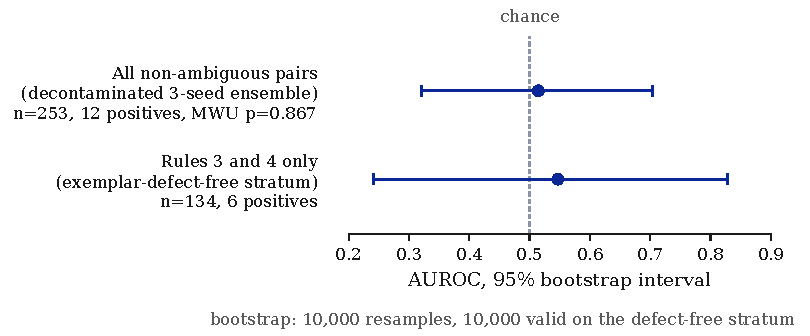
\includegraphics[width=0.92\linewidth]{figures/fig-disc-strata.pdf}
\caption{The measurement that closes the largest objection to
Chapter~\ref{ch:eval}. On the strata where the annotated evidence is correct by
construction, the detector's ranking is at chance rather than merely attenuated
toward it. The right panel rests on six positives and its interval is wide; the
claim it supports is that label contamination is not the explanation, not that
the true value is $0.5078$. Twenty of its $10{,}000$ resamples were dropped for
containing no positives, which is why the stratified band is shown alongside.}
\label{fig:disc-strata}
\end{figure}

\begin{figure}[t]
\centering
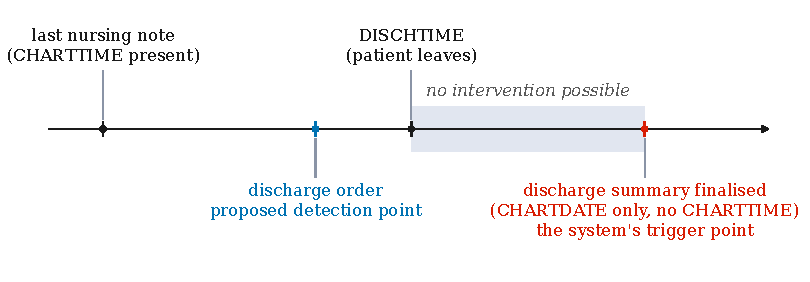
\includegraphics[width=0.92\linewidth]{figures/fig-disc-actionability.pdf}
\caption{The actionability flaw. The document that supplies one half of the
comparison does not exist until after the patient has left, so the prevention
story the design assumed is unavailable from this trigger. Either detection
moves to the discharge order, or the contribution is retrospective audit.}
\label{fig:disc-actionability}
\end{figure}

\section{Summary}
\label{sec:disc-summary}

Of the four research questions, one is answered negatively with a mechanism
(weak supervision cannot replace expert annotation here, because the labeller's
marginal is inverted by roughly $21\times$ and the student inherits it), one is
unaddressable in this resource (temporal ordering, because \texttt{CHARTTIME} is
null for every discharge summary), and two were never tested (authority
conditioning, whose parameter was initialised at the values reported as
discovered and sits where a normalisation erases it; and severity ranking, whose
component received no gradient).

The limitations are severe and are stated as such. $299$ annotated pairs against
a stated requirement of $548$. One annotator with no established inter-rater
reliability and a previously reported $\kappa$ of $1.000$ that is circular and
retracted. An exemplar selection defect affecting $41.4\%$ of action-conflict
candidates, which makes the measured $4.0\%$ precision an upper bound on
annotation validity rather than an estimate of pool quality. One institution, one
era, one primary cohort, retrospective throughout. No sub-day temporal ordering.
And a detection point that cannot precede the patient's departure, which is a
design flaw rather than a caveat and which forces a choice between moving
detection to the discharge order and reframing the contribution as retrospective
audit.

The central finding survives the most serious of these. On Rules 3 and 4, which
cannot exhibit the exemplar defect, the detector's AUROC is $0.5078$ with
Mann-Whitney $p = 0.953$ and a bootstrap $95\%$ interval of $[0.2217, 0.7615]$,
$[0.2643, 0.7344]$ when stratified. Six positives support that estimate, $20$ of
its $10{,}000$ resamples had to be discarded for containing none of them, and
both facts are stated rather than absorbed. It also survives a defect in the
reporting itself: the figures this thesis previously gave for the detector were
the contaminated configuration's, and the decontaminated retrain that replaces
them is worse on recall, precision, $F_1$ and $\kappa$.

The work that follows should start upstream of everything this project spent its
effort on: a better candidate generator, because $4.0\%$ precision is the binding
constraint and no downstream model repairs it; a weak labeller with a validated
operating point, or none; re-annotation of the $739$ candidates whose evidence
changed; a second annotator; and a second institution.
